% Options for packages loaded elsewhere
\PassOptionsToPackage{unicode}{hyperref}
\PassOptionsToPackage{hyphens}{url}
%
\documentclass[
]{article}
\usepackage{lmodern}
\usepackage{amssymb,amsmath}
\usepackage{ifxetex,ifluatex}
\ifnum 0\ifxetex 1\fi\ifluatex 1\fi=0 % if pdftex
  \usepackage[T1]{fontenc}
  \usepackage[utf8]{inputenc}
  \usepackage{textcomp} % provide euro and other symbols
\else % if luatex or xetex
  \usepackage{unicode-math}
  \defaultfontfeatures{Scale=MatchLowercase}
  \defaultfontfeatures[\rmfamily]{Ligatures=TeX,Scale=1}
\fi
% Use upquote if available, for straight quotes in verbatim environments
\IfFileExists{upquote.sty}{\usepackage{upquote}}{}
\IfFileExists{microtype.sty}{% use microtype if available
  \usepackage[]{microtype}
  \UseMicrotypeSet[protrusion]{basicmath} % disable protrusion for tt fonts
}{}
\makeatletter
\@ifundefined{KOMAClassName}{% if non-KOMA class
  \IfFileExists{parskip.sty}{%
    \usepackage{parskip}
  }{% else
    \setlength{\parindent}{0pt}
    \setlength{\parskip}{6pt plus 2pt minus 1pt}}
}{% if KOMA class
  \KOMAoptions{parskip=half}}
\makeatother
\usepackage{xcolor}
\IfFileExists{xurl.sty}{\usepackage{xurl}}{} % add URL line breaks if available
\IfFileExists{bookmark.sty}{\usepackage{bookmark}}{\usepackage{hyperref}}
\hypersetup{
  pdftitle={Conversion between Lux and Exposure Values},
  hidelinks,
  pdfcreator={LaTeX via pandoc}}
\urlstyle{same} % disable monospaced font for URLs
\usepackage[margin=1in]{geometry}
\usepackage{color}
\usepackage{fancyvrb}
\newcommand{\VerbBar}{|}
\newcommand{\VERB}{\Verb[commandchars=\\\{\}]}
\DefineVerbatimEnvironment{Highlighting}{Verbatim}{commandchars=\\\{\}}
% Add ',fontsize=\small' for more characters per line
\usepackage{framed}
\definecolor{shadecolor}{RGB}{248,248,248}
\newenvironment{Shaded}{\begin{snugshade}}{\end{snugshade}}
\newcommand{\AlertTok}[1]{\textcolor[rgb]{0.94,0.16,0.16}{#1}}
\newcommand{\AnnotationTok}[1]{\textcolor[rgb]{0.56,0.35,0.01}{\textbf{\textit{#1}}}}
\newcommand{\AttributeTok}[1]{\textcolor[rgb]{0.77,0.63,0.00}{#1}}
\newcommand{\BaseNTok}[1]{\textcolor[rgb]{0.00,0.00,0.81}{#1}}
\newcommand{\BuiltInTok}[1]{#1}
\newcommand{\CharTok}[1]{\textcolor[rgb]{0.31,0.60,0.02}{#1}}
\newcommand{\CommentTok}[1]{\textcolor[rgb]{0.56,0.35,0.01}{\textit{#1}}}
\newcommand{\CommentVarTok}[1]{\textcolor[rgb]{0.56,0.35,0.01}{\textbf{\textit{#1}}}}
\newcommand{\ConstantTok}[1]{\textcolor[rgb]{0.00,0.00,0.00}{#1}}
\newcommand{\ControlFlowTok}[1]{\textcolor[rgb]{0.13,0.29,0.53}{\textbf{#1}}}
\newcommand{\DataTypeTok}[1]{\textcolor[rgb]{0.13,0.29,0.53}{#1}}
\newcommand{\DecValTok}[1]{\textcolor[rgb]{0.00,0.00,0.81}{#1}}
\newcommand{\DocumentationTok}[1]{\textcolor[rgb]{0.56,0.35,0.01}{\textbf{\textit{#1}}}}
\newcommand{\ErrorTok}[1]{\textcolor[rgb]{0.64,0.00,0.00}{\textbf{#1}}}
\newcommand{\ExtensionTok}[1]{#1}
\newcommand{\FloatTok}[1]{\textcolor[rgb]{0.00,0.00,0.81}{#1}}
\newcommand{\FunctionTok}[1]{\textcolor[rgb]{0.00,0.00,0.00}{#1}}
\newcommand{\ImportTok}[1]{#1}
\newcommand{\InformationTok}[1]{\textcolor[rgb]{0.56,0.35,0.01}{\textbf{\textit{#1}}}}
\newcommand{\KeywordTok}[1]{\textcolor[rgb]{0.13,0.29,0.53}{\textbf{#1}}}
\newcommand{\NormalTok}[1]{#1}
\newcommand{\OperatorTok}[1]{\textcolor[rgb]{0.81,0.36,0.00}{\textbf{#1}}}
\newcommand{\OtherTok}[1]{\textcolor[rgb]{0.56,0.35,0.01}{#1}}
\newcommand{\PreprocessorTok}[1]{\textcolor[rgb]{0.56,0.35,0.01}{\textit{#1}}}
\newcommand{\RegionMarkerTok}[1]{#1}
\newcommand{\SpecialCharTok}[1]{\textcolor[rgb]{0.00,0.00,0.00}{#1}}
\newcommand{\SpecialStringTok}[1]{\textcolor[rgb]{0.31,0.60,0.02}{#1}}
\newcommand{\StringTok}[1]{\textcolor[rgb]{0.31,0.60,0.02}{#1}}
\newcommand{\VariableTok}[1]{\textcolor[rgb]{0.00,0.00,0.00}{#1}}
\newcommand{\VerbatimStringTok}[1]{\textcolor[rgb]{0.31,0.60,0.02}{#1}}
\newcommand{\WarningTok}[1]{\textcolor[rgb]{0.56,0.35,0.01}{\textbf{\textit{#1}}}}
\usepackage{graphicx,grffile}
\makeatletter
\def\maxwidth{\ifdim\Gin@nat@width>\linewidth\linewidth\else\Gin@nat@width\fi}
\def\maxheight{\ifdim\Gin@nat@height>\textheight\textheight\else\Gin@nat@height\fi}
\makeatother
% Scale images if necessary, so that they will not overflow the page
% margins by default, and it is still possible to overwrite the defaults
% using explicit options in \includegraphics[width, height, ...]{}
\setkeys{Gin}{width=\maxwidth,height=\maxheight,keepaspectratio}
% Set default figure placement to htbp
\makeatletter
\def\fps@figure{htbp}
\makeatother
\setlength{\emergencystretch}{3em} % prevent overfull lines
\providecommand{\tightlist}{%
  \setlength{\itemsep}{0pt}\setlength{\parskip}{0pt}}
\setcounter{secnumdepth}{-\maxdimen} % remove section numbering

\title{Conversion between Lux and Exposure Values}
\author{}
\date{\vspace{-2.5em}}

\begin{document}
\maketitle

\textbf{\emph{How to determine exposure from LED panels Lux
specifications, for photographers}}

LED panels are getting cheaper and more readily available and
photographers may consider using them as a substitute to strobes. Here I
am talking about the small, battery powered panels normally used by
videographers, not the big continuous lights used in photography studios
or film sets. These panels are the size and weight of small strobe units
and can be mounted on the camera hot shoe. In fact the form factor is
quite convenient, being very similar to smarphones. And additionally,
they work independently form the camer system, so, for instance, they
can be used to vintage film cameras equipped with only a ``cold shoe''.

The downside of these units is that they are far less powerful than
strobes of equivalent size. However, determining the light output
generated by these lights in units of measure typically used in
photography is not straightforward. Indeed, LED panes' specifications
for what concearns light ouput are normally expressed in Lux (lx)
measured at a certain distance from the source. When considering whether
a specific LED panel would be of much use for a photographer, it would
be useful to know the Exposure Value (EV) that corresponds to the
panel's' specification: what ISO, shutter speed and aperture values are
needed to correctly expose an object illuminated by the panel from a
given distance?

Luckily, we can convert between EV and lx. That is to say that it is
possible to determine the photographic exposure necessary to photograph
an object receiving a given amount of light expressed in lx. The
conversio formula found on
\href{http://en.wikipedia.org/wiki/Exposure_value\#EV_as_a_measure_of_luminance_and_illuminance}{Wikipedia}
is simple:

\includegraphics{https://wikimedia.org/api/rest_v1/media/math/render/svg/c276b05aae70d59e4b5d3fd6816efd74503d9bfc}

Where ``\emph{E}'' is illuminance in Lux, and ``EV'' is the Exposure
Value at iso 100 (this corresponds to the Light Value (LV)).

I was interested in the a very portable panel for use in
macrophotography, as a fill light in portraits (quite rarely) or as a
main light for a portrait-range, dark scene. An example of such tool is
the \href{https://lumecube.com/products/panel-go}{Lume Cube Light Go}
which is rated at 1080 lx measured 0.5 metres away. I wanted to know if
I could use such a light for the above scenes. To take the most
demanding one (i.e.~as main light), I would like to know if it can give
me enough light to shoot hand-held when focussing at 1 m with ISO 400
film and a 50 mm f:2.8 lens. With my film SLR I can hand-hold sharp
shots with a 50mm down to 1/60''. This means LV7 or EV9 at ISO 400.

To do so, I set up some R code with the conversion functions:

\begin{Shaded}
\begin{Highlighting}[]
\CommentTok{# From Light Values to Lux}
\NormalTok{lv2lux <-}\StringTok{ }\ControlFlowTok{function}\NormalTok{(lv) (}\DecValTok{2}\OperatorTok{^}\NormalTok{lv)}\OperatorTok{*}\FloatTok{2.5}  

\CommentTok{# From Lux to Light Values}
\NormalTok{lux2lv <-}\StringTok{ }\ControlFlowTok{function}\NormalTok{(lux) }\KeywordTok{log}\NormalTok{(lux}\OperatorTok{/}\FloatTok{2.5}\NormalTok{, }\DecValTok{2}\NormalTok{)}
\end{Highlighting}
\end{Shaded}

And plotted the curve from LV5 to lv11, which represent dark settings in
which flash would be useful. Since light intensity is inversely
proportional to the square of the distance (inverse square law) if the
distance doubles, the light intensity drops by two stops (25\% of
intensity at original distance). So, if the panel generates 1080 lx at
0.5 m, it would generate a fourth of that (270 lx) at 1 m. What is the
corresponding LV of this? We can see from the curve (and from the code)
it is a quarter of a stop less than LV7 (LV6.75).

This means that by keeping the panel on-camera, I could just barely
expose for an object at 1 m away, 1.5 m if I had an f:2 lense, or if I
could hand-hold 1/30'`, and 2 m if I had an f:2 lense \textbf{and} I
could hand-hold 1/30''.

\begin{Shaded}
\begin{Highlighting}[]
\CommentTok{# Interactive plot}

\NormalTok{lv <-}\StringTok{ }\KeywordTok{seq}\NormalTok{(}\DecValTok{5}\NormalTok{,}\DecValTok{11}\NormalTok{,.}\DecValTok{5}\NormalTok{)}
\NormalTok{lux <-}\StringTok{ }\KeywordTok{lv2lux}\NormalTok{(lv)}
\KeywordTok{plot}\NormalTok{(lv, lux, }\DataTypeTok{type =} \StringTok{"l"}\NormalTok{,}
     \DataTypeTok{xlab =} \StringTok{"Light Values [LV]"}\NormalTok{, }\DataTypeTok{ylab =} \StringTok{"Lux [lx]"}\NormalTok{,}
     \DataTypeTok{col =} \StringTok{"red"}\NormalTok{)}
\KeywordTok{points}\NormalTok{(}\KeywordTok{lux2lv}\NormalTok{(}\DecValTok{1080}\OperatorTok{/}\DecValTok{4}\NormalTok{), }\DecValTok{1080}\OperatorTok{/}\DecValTok{4}\NormalTok{, }\DataTypeTok{col =} \StringTok{"blue"}\NormalTok{)}
\KeywordTok{text}\NormalTok{(}\KeywordTok{lux2lv}\NormalTok{(}\DecValTok{1080}\OperatorTok{/}\DecValTok{4}\NormalTok{), }\DecValTok{1080}\OperatorTok{/}\DecValTok{4}\NormalTok{, }\DataTypeTok{col =} \StringTok{"blue"}\NormalTok{,}
     \DataTypeTok{labels =} \KeywordTok{paste0}\NormalTok{(}\StringTok{"LV"}\NormalTok{, }\KeywordTok{round}\NormalTok{(}\KeywordTok{lux2lv}\NormalTok{(}\DecValTok{1080}\OperatorTok{/}\DecValTok{4}\NormalTok{), }\DecValTok{2}\NormalTok{), }\StringTok{", "}\NormalTok{, }\DecValTok{1080}\OperatorTok{/}\DecValTok{4}\NormalTok{, }\StringTok{" lx"}\NormalTok{),}
     \DataTypeTok{adj =} \KeywordTok{c}\NormalTok{(}\DecValTok{1}\NormalTok{,}\OperatorTok{-}\DecValTok{1}\NormalTok{))}
\end{Highlighting}
\end{Shaded}

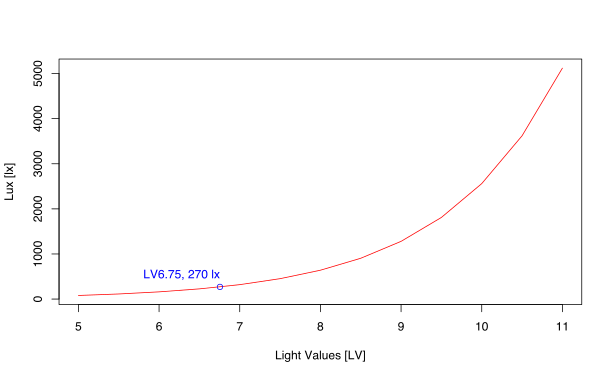
\includegraphics{2021-01-31-Switching-between-LUX-and-exposure-values_files/figure-latex/plot-1.pdf}
To conclude, the \href{https://lumecube.com/products/panel-go}{Lume Cube
Light Go}, or any other LED panel of similar power, may just be usefull
in very limited circumstances, and not really be able to subtitue a
strobe for most of the uses a strobe is normally used for\ldots{}

\end{document}
